\section{PMT Studies}

\subsection{PMT Magnetic Shielding Studies}

The PMTs of the HTCC will be located in a region in which there will 
be a significant magnetic field, primarily from the solenoid magnet 
that surrounds the target and central detector system.  The field 
varies considerably with distance from the solenoid, with a maximum 
value of as much as 50~G in the region of the PMTs closest to the 
solenoid.  To give an idea of the magnitude of the problem, we note 
that for tests we have carried out, the PMT gain is reduced by a factor
of two for a magnetic field of 0.4~G perpendicular to the PMT axis    
and 1.3~G parallel to the PMT axis.  The standard PMT magnetic shield 
that can be obtained from the PMT manufacturer is totally inadequate to 
reduce the ambient field to even these levels, so that it is necessary 
to custom design a magnetic shielding system appropriate for the
{\tt CLAS12} HTCC configuration.  The design is being carried out with 
the aid of the TOSCA magnetic field program. 

Figs.~\ref{lin_r}, \ref{log_r}, \ref{lin_z}, and \ref{log_z} present the 
residual magnetic field at the PMT axis for a standard single-layer PMT 
magnetic shield for three values of the field: 50~G, 40~G, and 30~G, 
with the direction of the magnetic field perpendicular and parallel to the 
PMT axis (linear and logarithmic $y$-scales are shown).  In the first 
case, the residual magnetic field inside the PMT volume is around 8~G, 
2~G, and 1~G for a magnetic field of 50~G, 40~G, and 30~G, respectively. 
For the second case (the field is along the PMT axis), the field residual 
is significantly higher.  The residual magnetic field inside the PMT volume 
is around 30~G, 10~G, and 1-2~G for magnetic fields of 50~G, 40~G, and 
30~G, respectively.  We may conclude from this calculation that:

\begin{itemize}
\item We need additional magnetic shielding to suppress the residual 
magnetic field to the level of 0.5~G;
\item The residual field is significantly (several times) higher when 
the magnetic field is directed along the PMT axis;
\item The shielding needs to extend beyond the PMT window for at least 
one PMT diameter.
\end{itemize}

We modeled three-layer magnetic shielding configurations using the 
TOSCA program.  Fig.~\ref{3layers} shows the residual field for 3 
different configurations with cylindrical PMT magnetic shielding with 
the magnetic field directed along the PMT axis.  The magnetic shielding 
has 1-mm thickness for every layer.  For these studies, the following
conditions apply:

\begin{itemize}
\item Single layer tube made of co-netic $\mu$-metal (shown in black),
\item Two layers made of netic and co-netic $\mu$-metals (shown in red),
\item Three layers made of netic, co-netic, and co-netic $\mu$-metals 
(shown in blue).
\end{itemize}

The residual magnetic field with the three-layer shielding is below 1~G 
in the region $\pm$5~cm, which is inside the specifications for the
magnetic field parallel to the PMT axis.  The perpendicular field will 
be several times lower, based on our calculations with the standard PMT 
magnetic shielding.

%%%%%%%%%%%%%%%%%%%%%%%%%%%%%%%%%%%%%%%%%%%%%%%%%%%%%%%%%%%%%%%%%%%%%%%%
\begin{figure}
\hspace{0.5cm}
\begin{centering}
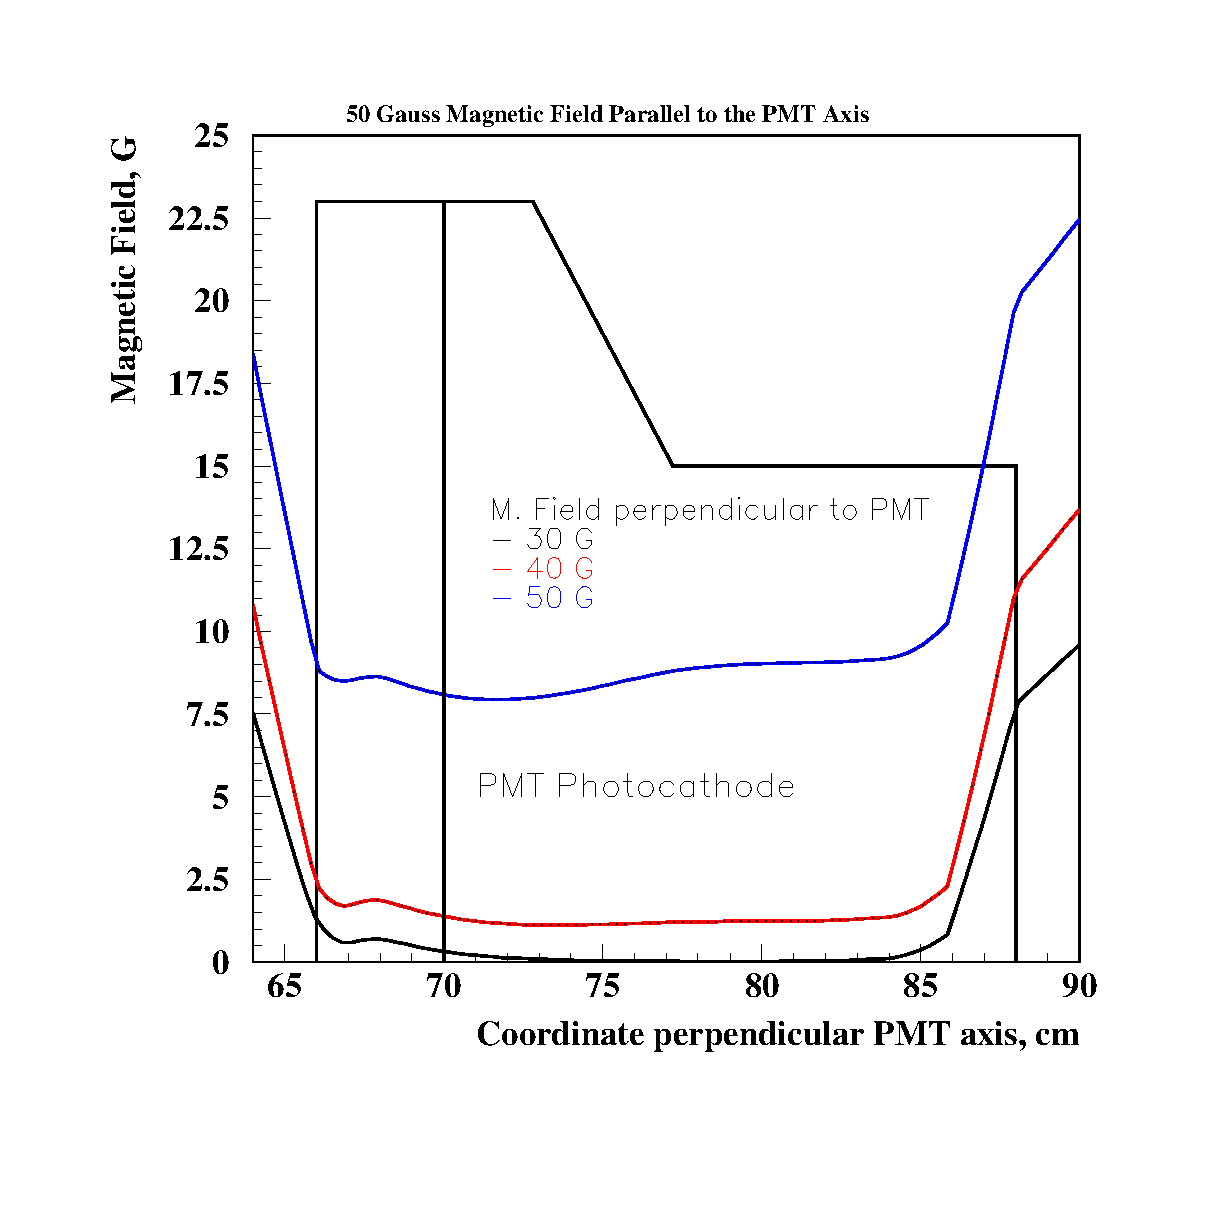
\includegraphics[height=7.5cm]{Magnetic-shielding/shield_r_lin.eps}
\vspace{0.5cm}
\caption{\small{Standard single-layer PMT magnetic shielding (shown in 
black).  The magnetic field is perpendicular to the PMT axis.  The result 
with applied external fields of 50~G is shown in blue, 40~G in red, and 
30~G in black.  The PMT photocathode position is shown by the black 
vertical line.}}
\label{lin_r}
\end{centering}
\end{figure}
%%%%%%%%%%%%%%%%%%%%%%%%%%%%%%%%%%%%%%%%%%%%%%%%%%%%%%%%%%%%%%%%%%%%%%%%

%%%%%%%%%%%%%%%%%%%%%%%%%%%%%%%%%%%%%%%%%%%%%%%%%%%%%%%%%%%%%%%%%%%%%%%%
\begin{figure}
\hspace{0.5cm}
\begin{centering}
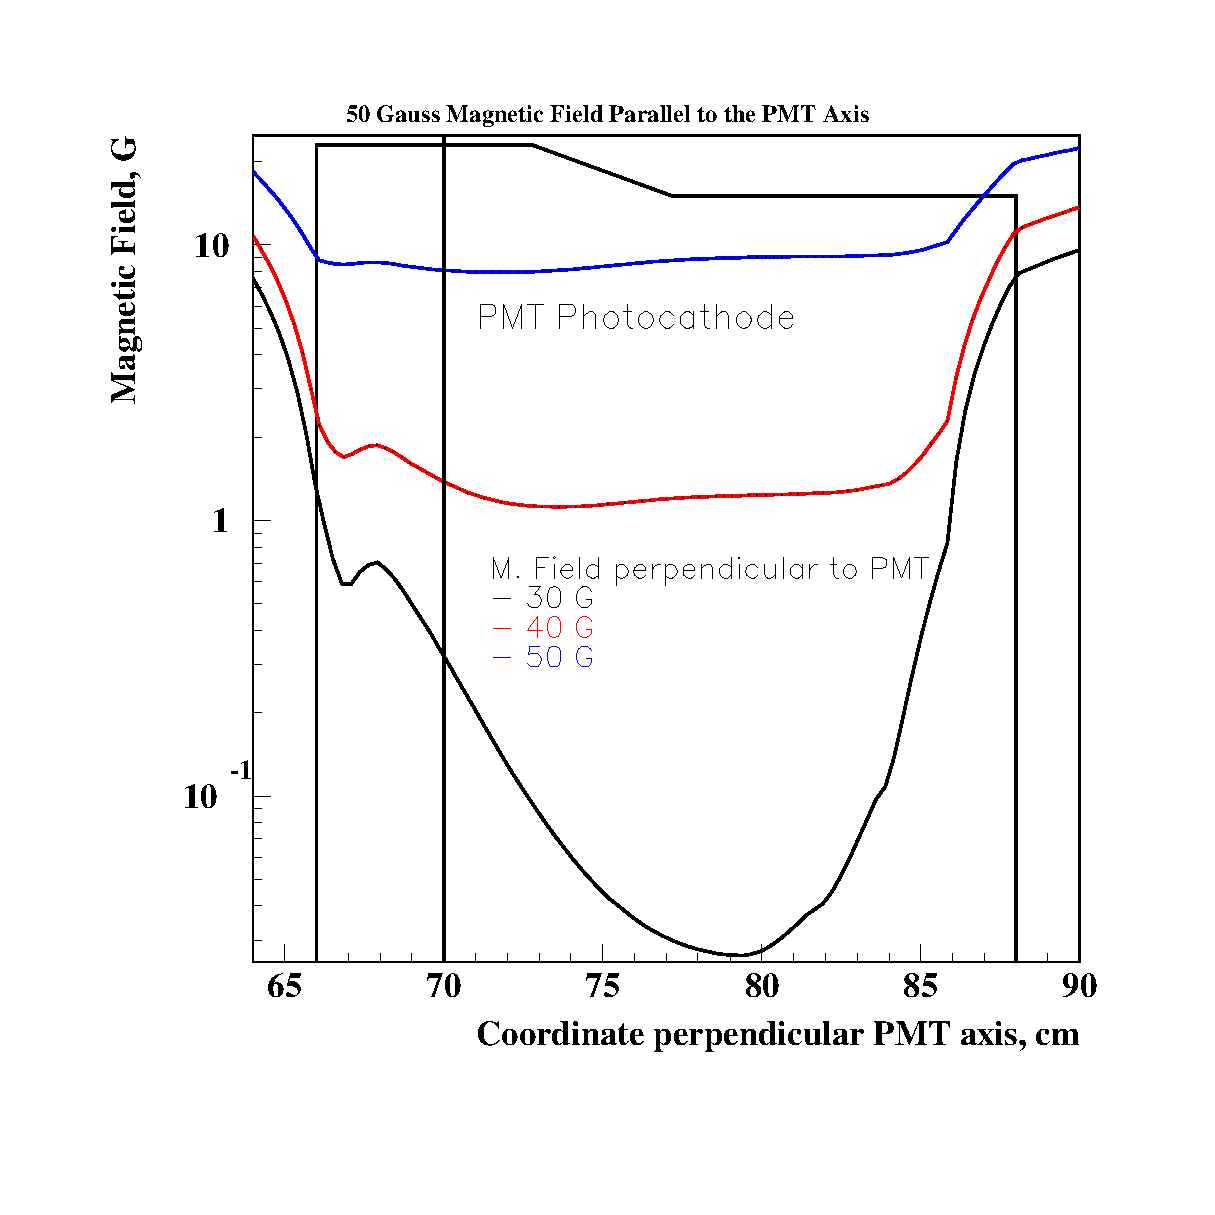
\includegraphics[height=7.5cm]{Magnetic-shielding/shield_r_log.eps}
\vspace{0.5cm}
\caption{\small{Same as in Fig.~\ref{lin_r} but with a logarithmic $y$-axis.
The PMT photocathode position is shown by the black vertical line.}}
\label{log_r}
\end{centering}
\end{figure}
%%%%%%%%%%%%%%%%%%%%%%%%%%%%%%%%%%%%%%%%%%%%%%%%%%%%%%%%%%%%%%%%%%%%%%%%

%%%%%%%%%%%%%%%%%%%%%%%%%%%%%%%%%%%%%%%%%%%%%%%%%%%%%%%%%%%%%%%%%%%%%%%%
\begin{figure}
\hspace{0.5cm}
\begin{centering}
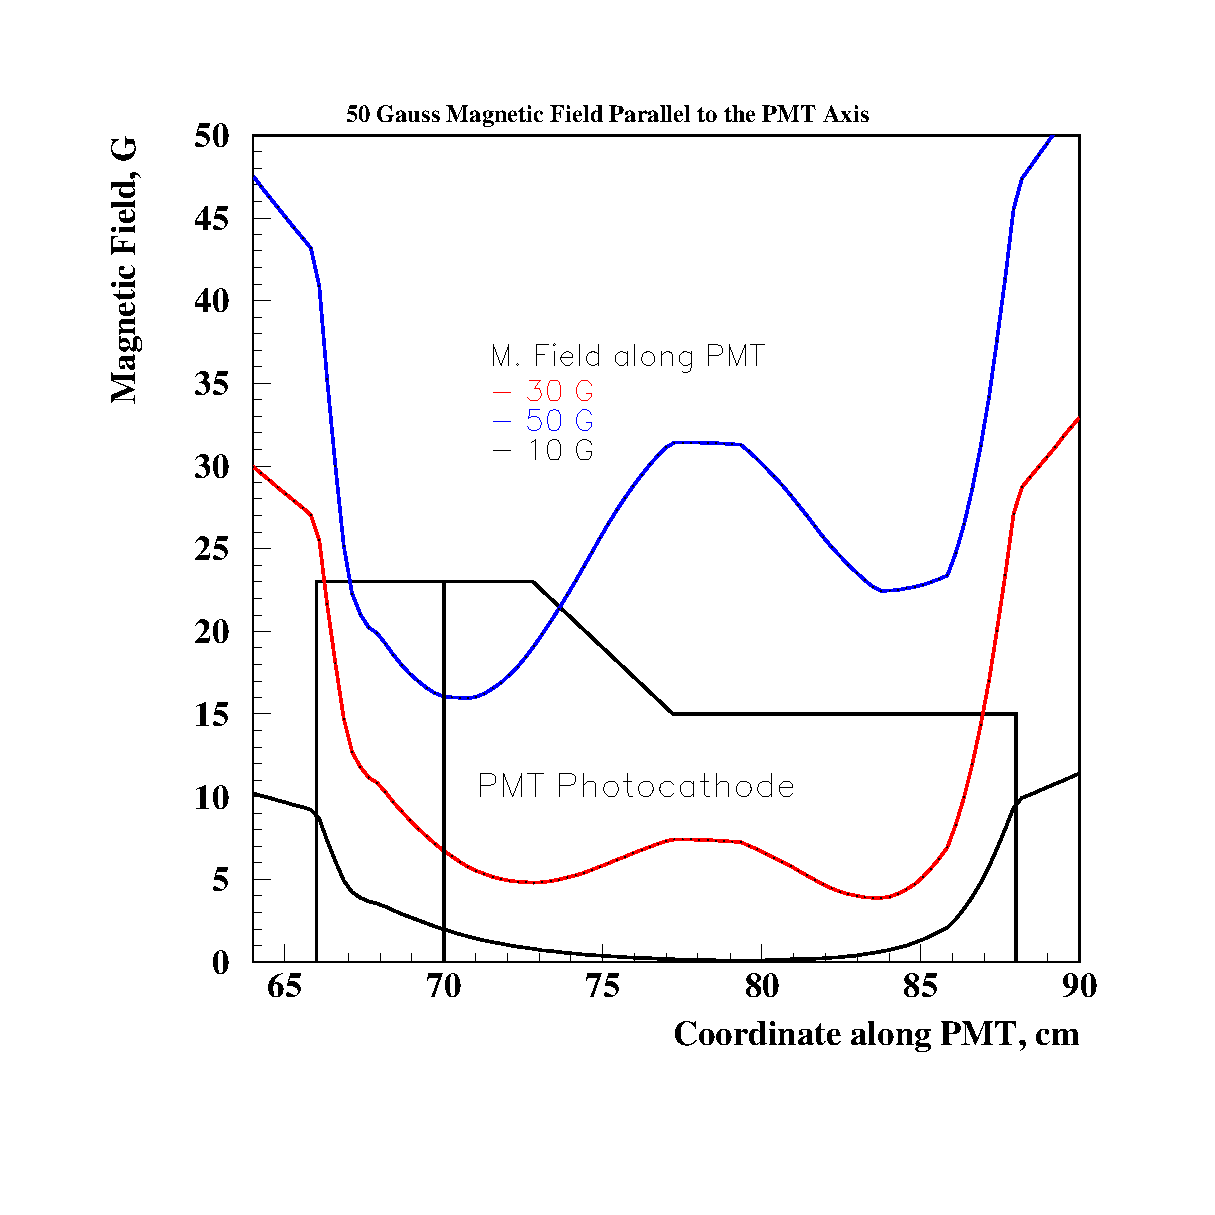
\includegraphics[height=7.5cm]{Magnetic-shielding/shield_z_lin.eps}
\vspace{0.5cm}
\caption{\small{Standard single-layer PMT magnetic shielding (shown in black).
The applied magnetic field is along the PMT axis: 50~G is shown in blue, 
40~G in red, and 30~G in black.  The PMT photocathode position is shown by 
the black the vertical line.}}
\label{lin_z}
\end{centering}
\end{figure}
%%%%%%%%%%%%%%%%%%%%%%%%%%%%%%%%%%%%%%%%%%%%%%%%%%%%%%%%%%%%%%%%%%%%%%%%

%%%%%%%%%%%%%%%%%%%%%%%%%%%%%%%%%%%%%%%%%%%%%%%%%%%%%%%%%%%%%%%%%%%%%%%%
\begin{figure}
\hspace{0.5cm}
\begin{centering}
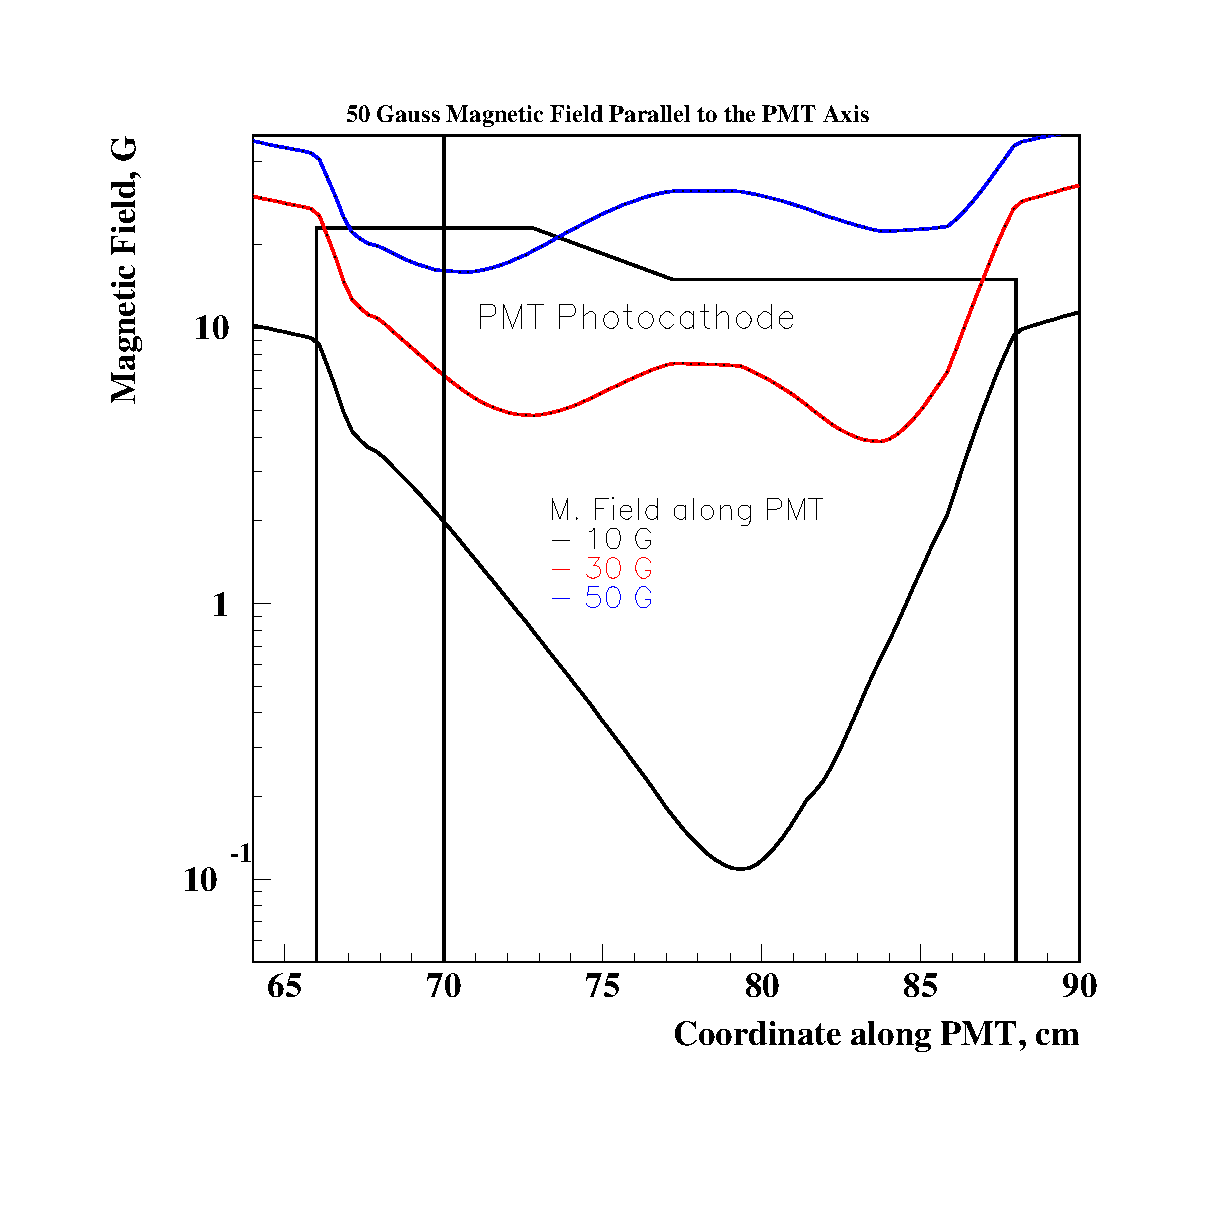
\includegraphics[height=7.5cm]{Magnetic-shielding/shield_z_log.eps}
\vspace{0.5cm}
\caption{\small{Same as Fig.~\ref{lin_z} but with a logarithmic $y$-axis.}}
\label{log_z}
\end{centering}
\end{figure}
%%%%%%%%%%%%%%%%%%%%%%%%%%%%%%%%%%%%%%%%%%%%%%%%%%%%%%%%%%%%%%%%%%%%%%%%

%%%%%%%%%%%%%%%%%%%%%%%%%%%%%%%%%%%%%%%%%%%%%%%%%%%%%%%%%%%%%%%%%%%%%%%%
\begin{figure}
\hspace{0.5cm}
\begin{centering}
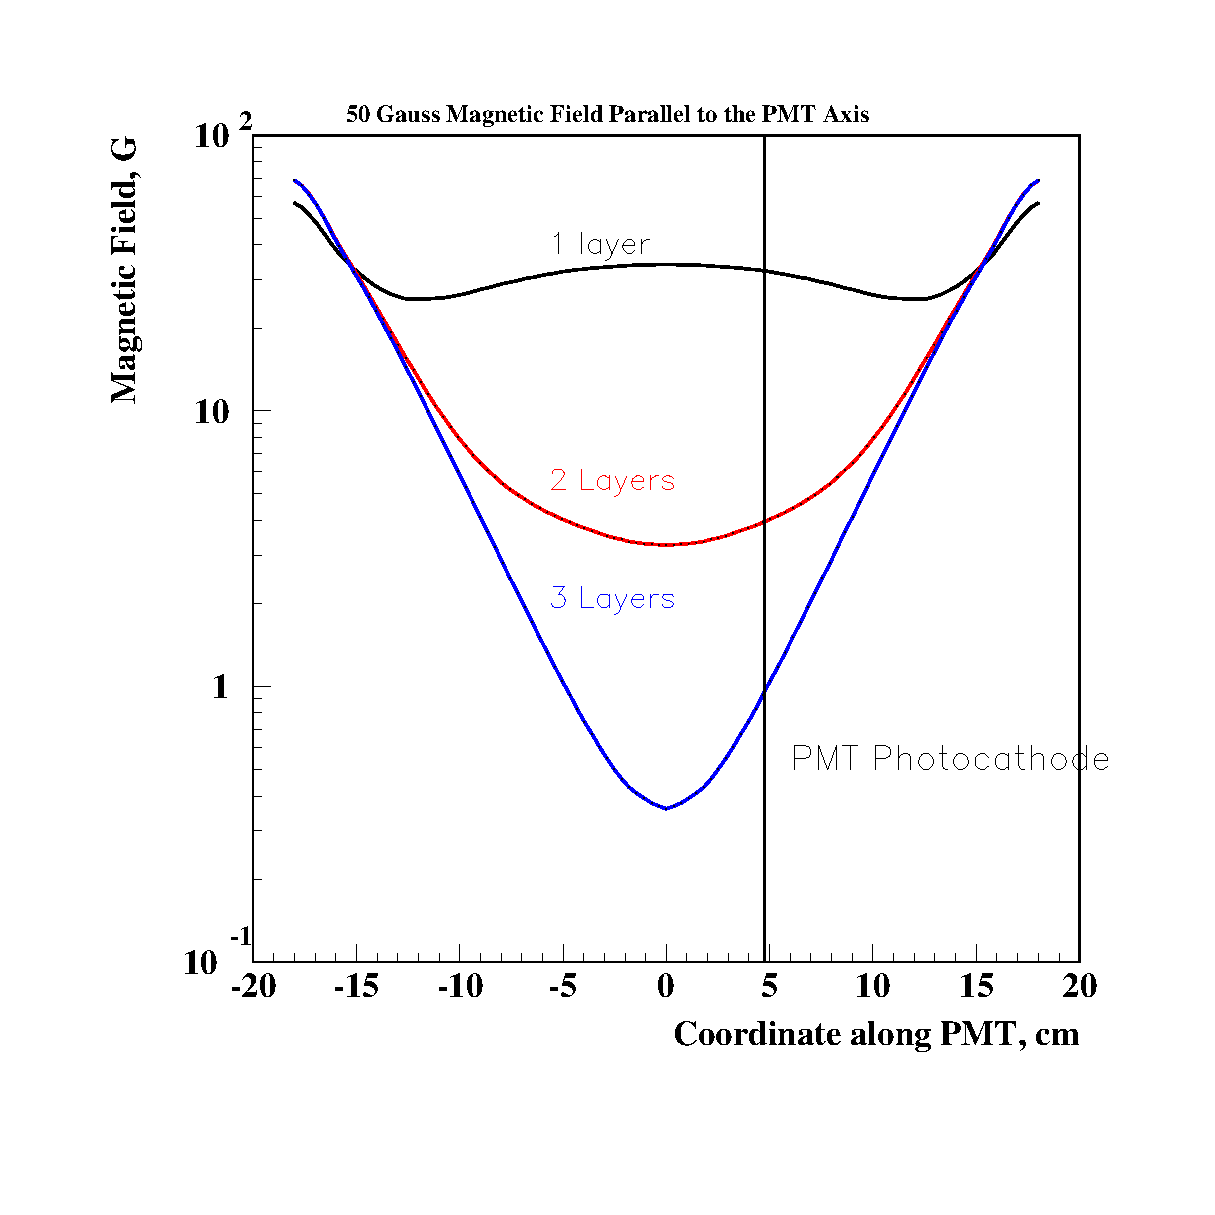
\includegraphics[height=7.5cm]{Magnetic-shielding/3layers.eps}
\vspace{0.5cm}
\caption{\small{The effect of cylindrical PMT magnetic shielding, in which
the applied magnetic field is 20~G along the PMT axis. Single-layer shielding 
is shown in black, two-layer shielding is shown in red, and three-layer
shielding is shown in blue.  The PMT photocathode position is shown by 
the black vertical line.}}
\label{3layers}
\end{centering}
\end{figure}
%%%%%%%%%%%%%%%%%%%%%%%%%%%%%%%%%%%%%%%%%%%%%%%%%%%%%%%%%%%%%%%%%%%%%%%%

\subsection{Magnetic Shielding Test Stand}

A test stand (Fig.~\ref{magstand}) was used to study the magnetic 
shielding properties.  The magnetic shielding was placed inside a black 
box that is located between two circular magnetic coils that produce an 
external magnetic field.  A high-current power supply allows us to vary 
the current up to 107~A, which corresponds to a magnetic field value of 
68~G.  The calibration line showing the relation between current and the 
magnetic field is shown in Fig.~\ref{magcalibration}.  We have measured 
the magnetic field along the PMT axis inside the shielding by using the 
Gauss/Teslameter (Model 5070) measuring device. The results of the 
measurements for the single shielding layers are shown in 
Fig.~\ref{magshield1}.  Note that the first shielding layer is a prototype 
shield that was ordered for testing from the manufacturer.  It is a 
cylindrical magnetic shield, 50\% alloy of NiFe with a 6.19-in outer 
diameter, 6.06-in inner diameter, and 18.7-in long.  The second shield layer 
is a standard PMT magnetic shield.  Fig.~\ref{prototype-shielding} shows a 
drawing of the PMT and Winston Cone inserted inside the prototype shield. 
Results of the measurements for the double-layer shielding are shown in 
Fig.~\ref{magshield2}.  According to Fig.~\ref{magshield2}, we expect a
0.3~G magnetic field on the PMTs with the two-layer shield in a nominal 
30~G external magnetic field.  Studies of the PMT performance affected 
by different magnetic field conditions are underway.

%%%%%%%%%%%%%%%%%%%%%%%%%%%%%%%%%%%%%%%%%%%%%%%%%%%%%%%%%%%%%%%%%%%%%%%%
\begin{figure}
\hspace{0.5cm}
\begin{centering}
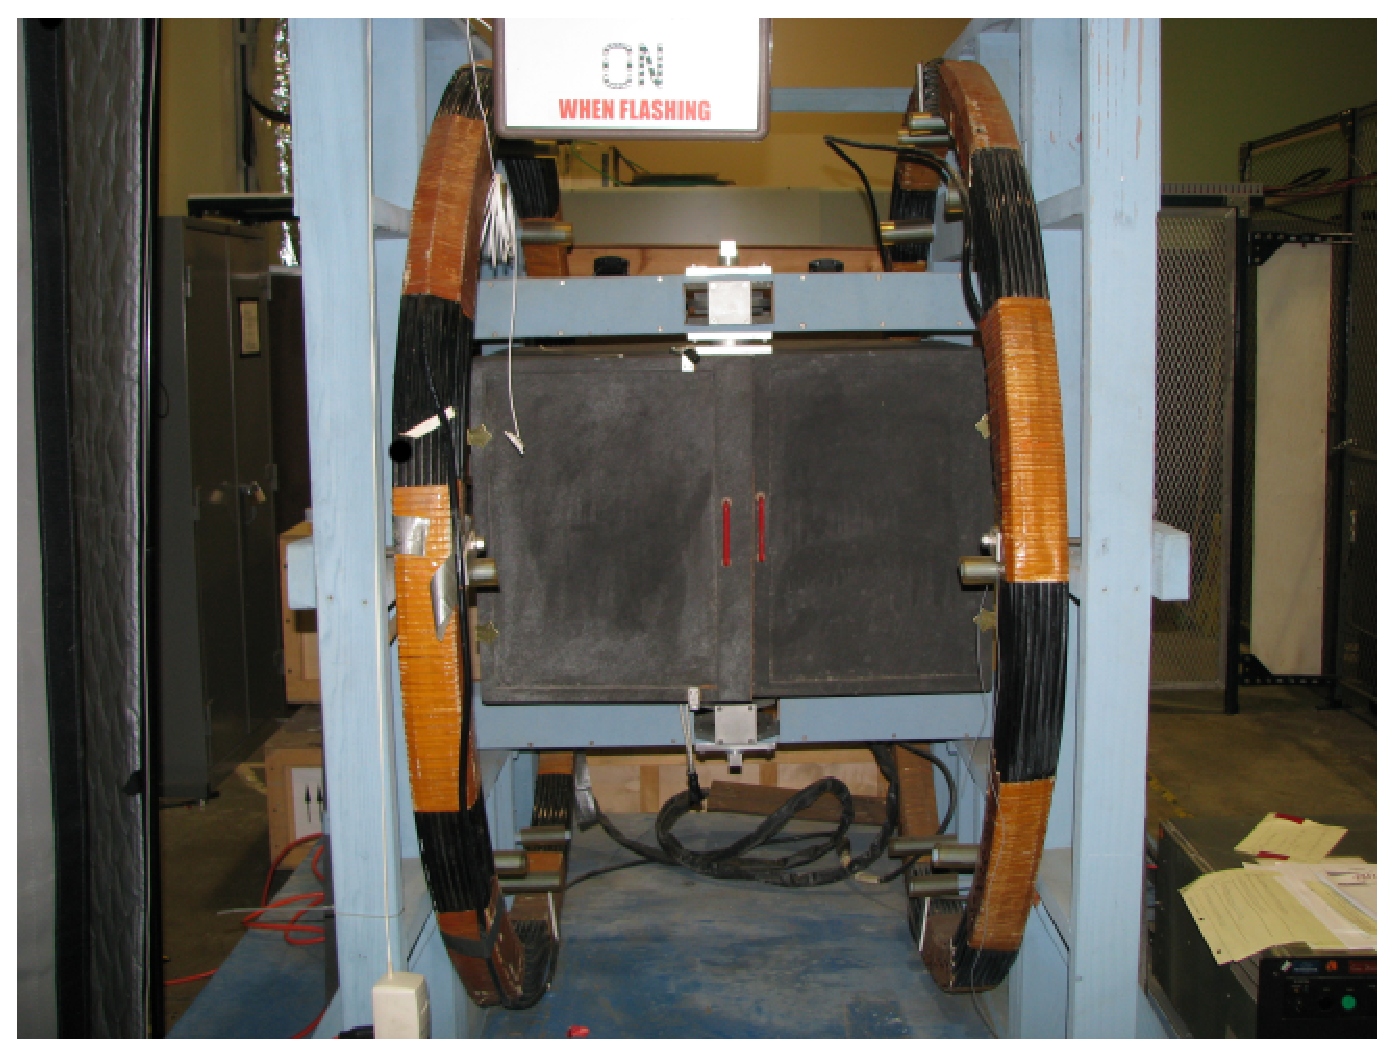
\includegraphics[height=7.5cm]{Magnetic-shielding/mag_stand.eps}
\vspace{0.5cm}
\caption{\small{Photograph of the magnetic shielding test stand.  The 
black box that contains the test shielding is located between the 
magnetic coils.}}
\label{magstand}
\end{centering}
\end{figure}
%%%%%%%%%%%%%%%%%%%%%%%%%%%%%%%%%%%%%%%%%%%%%%%%%%%%%%%%%%%%%%%%%%%%%%%%

%%%%%%%%%%%%%%%%%%%%%%%%%%%%%%%%%%%%%%%%%%%%%%%%%%%%%%%%%%%%%%%%%%%%%%%%
 \begin{figure}
 \hspace{0.5cm}
 \begin{centering}
  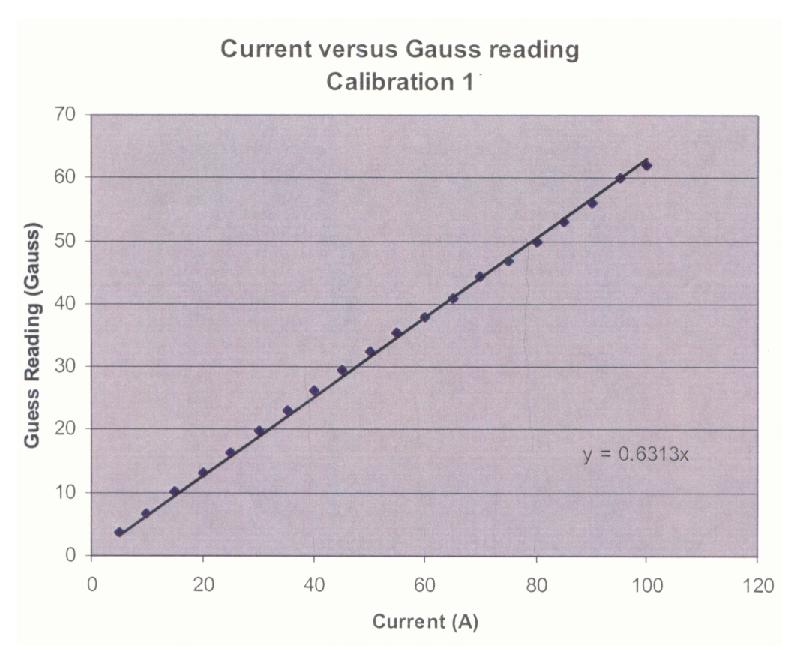
\includegraphics[height=7.5cm]{Magnetic-shielding/mag_calibration.eps}
 \vspace{0.5cm}
 \caption{\small{The current to magnetic field value calibration curve.}}
\label{magcalibration}
\end{centering}
 \end{figure}
%%%%%%%%%%%%%%%%%%%%%%%%%%%%%%%%%%%%%%%%%%%%%%%%%%%%%%%%%%%%%%%%%%%%%%%%

%%%%%%%%%%%%%%%%%%%%%%%%%%%%%%%%%%%%%%%%%%%%%%%%%%%%%%%%%%%%%%%%%%%%%%%%
 \begin{figure}
 \vspace{1.cm}
 \begin{centering}
  \includegraphics[height=7.5cm,angle=0]{Magnetic-shielding/magshield1.eps}
 \includegraphics[height=7.5cm,angle=0]{Magnetic-shielding/magshield2.eps}
 \hspace{0.1cm}
 \caption{\small{Results of the measurements of the magnetic field along 
the PMT axis inside the single-layer shield.  Left panel: The cylindrical 
shielding.  Right panel: The conventional PMT shielding.}}
\label{magshield1}
 \end{centering}
 \end{figure}
%%%%%%%%%%%%%%%%%%%%%%%%%%%%%%%%%%%%%%%%%%%%%%%%%%%%%%%%%%%%%%%%%%%%%%%%

%%%%%%%%%%%%%%%%%%%%%%%%%%%%%%%%%%%%%%%%%%%%%%%%%%%%%%%%%%%%%%%%%%%%%%%%
\begin{figure}
\hspace{0.5cm}
\begin{centering}
\includegraphics[height=10cm,angle=-90]{Magnetic-shielding/mag_shield.eps}
\vspace{0.5cm}
\caption{\small{Assembly of a photomultiplier tube with a Winston Cone 
magnetic shield.}}
\label{prototype-shielding}
\end{centering}
\end{figure}
%%%%%%%%%%%%%%%%%%%%%%%%%%%%%%%%%%%%%%%%%%%%%%%%%%%%%%%%%%%%%%%%%%%%%%%%

%%%%%%%%%%%%%%%%%%%%%%%%%%%%%%%%%%%%%%%%%%%%%%%%%%%%%%%%%%%%%%%%%%%%%%%%
 \begin{figure}
 \hspace{0.5cm}
 \begin{centering}
  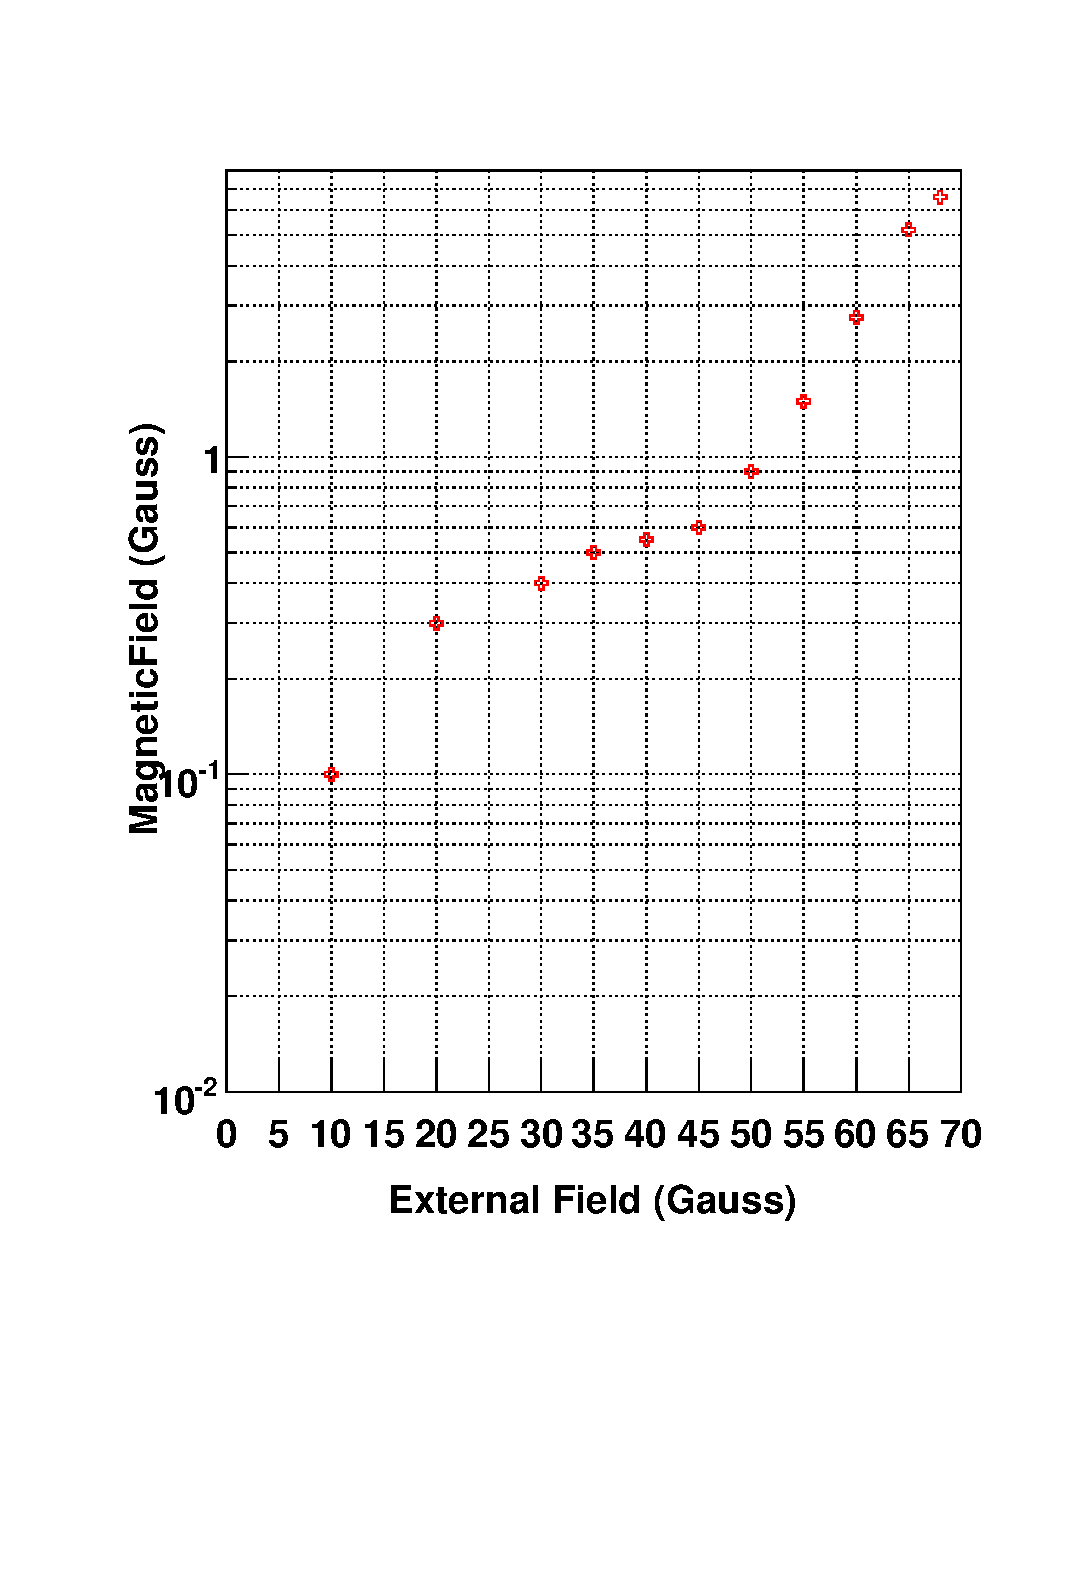
\includegraphics[height=9.5cm]{Magnetic-shielding/magshield3.eps}
 \vspace{0.5cm}
 \caption{\small{Results of the measurements of the magnetic field along 
the PMT axis inside the double-layer shield combined from the two single 
layers shown in Fig.~\ref{magshield1}.}}  
\label{magshield2}
\end{centering}
 \end{figure}
%%%%%%%%%%%%%%%%%%%%%%%%%%%%%%%%%%%%%%%%%%%%%%%%%%%%%%%%%%%%%%%%%%%%%%%%
